
\pdfminorversion=4

% Modos:
% Definir el comando \handoutmode como "1" para compilar las diapositivas en
% modo handout
% al pdf generado ejecutarle el siguiente comando para poner varias diapo en una misma pagina:
%    pdfnup FILE.pdf --nup 2x3 --no-landscape --paper letterpaper --frame True
%
% Definir \handoutmode como algo distinto de "1" para compilar las diapositivas
% normalmente.
%
% Para configurar el modo desde afuera (la linea de comandos de latex) correr
% la compilacion como:
%
%   latex -output-directory=tmp -output-format=pdf '\def\handoutmode{1}\include{FILE.tex}'
%
\if\handoutmode1
    \documentclass[professionalfonts,handout]{beamer}
    \setbeameroption{show notes}
    \setbeamertemplate{note page}{\insertnote}
    \setbeamercolor{background canvas}{bg=white}
\else
    \documentclass[professionalfonts]{beamer}
\fi


% Template original the Beamer: Copyright 2004 by Till Tantau <tantau@users.sourceforge.net>.


\mode<presentation>
{
  \usetheme{metropolis}
  % or ...

  %\setbeamercovered{transparent} %hace que lo que esta covered se muestre transparente
}

\setbeamertemplate{navigation symbols}{}%remove navigation symbols

\usepackage[english]{babel}

\usepackage[latin1]{inputenc}

\usepackage{times}
\usepackage[T1]{fontenc}

% para poder escribir codigo fuente en las diapositivas
\usepackage{listings}

% para graficar diagramas simples y arboles de jerarquias
\usepackage{tikz}
\usepackage{tikz-qtree}
\usetikzlibrary{matrix,positioning}
\usetikzlibrary{shapes,arrows,chains,calc,decorations.pathmorphing}

\usepackage{xcolor}
\definecolor{darkgreen}{rgb}{0,.5,0}
\definecolor{darkblue}{rgb}{0,0,.7}
\lstdefinestyle{normal}{language=C++,       % lenguaje C++
   numbers=left,                            % enumerar las lineas
   keywordstyle=\color{darkblue}\textbf,    % color de las keywords
   stringstyle=\color{red},                 % color de los strings
   commentstyle=\color{darkgreen},          % color de los comentarios
   basicstyle=\color{black}\ttfamily\footnotesize\bfseries,     % color del texto en general
   morecomment=[l][\color{magenta}]{\#},    % coloreamos las intrucciones del precompilador (todo lo que empieza con #)
   ndkeywords={NULL,nullptr,siz,zer,mov,add},               % definimos una nuevas keywords como NULL y nullptr
   ndkeywordstyle=\color{violet},           % y las nuevas keywords tendran este color
   frame=simple,                            % simple, sin ningun marco o frame alrededor del codigo
   basewidth={0.55em,0.55em}                % tamano de las letras/lineas. usado para reducir el whitespace entre estas
}

\lstdefinestyle{normal33}{language=C++,       % lenguaje C++
   numbers=left,                            % enumerar las lineas
   keywordstyle=\color{darkblue}\textbf,    % color de las keywords
   stringstyle=\color{red},                 % color de los strings
   commentstyle=\color{darkgreen},          % color de los comentarios
   basicstyle=\color{black}\ttfamily\footnotesize\bfseries,     % color del texto en general
   morecomment=[l][\color{magenta}]{\#},    % coloreamos las intrucciones del precompilador (todo lo que empieza con #)
   ndkeywords={NULL,nullptr},               % definimos una nuevas keywords como NULL y nullptr
   ndkeywordstyle=\color{violet},           % y las nuevas keywords tendran este color
   frame=simple,                            % simple, sin ningun marco o frame alrededor del codigo
   basewidth={0.55em,0.55em}                % tamano de las letras/lineas. usado para reducir el whitespace entre estas
}
%mismo estilo, sin numeros
\lstdefinestyle{normalnonumbers}{language=C++,
   keywordstyle=\color{darkblue}\textbf,
   stringstyle=\color{red},           
   commentstyle=\color{darkgreen},    
   basicstyle=\color{black}\ttfamily\footnotesize\bfseries,
   morecomment=[l][\color{magenta}]{\#},
   ndkeywords={NULL,nullptr,move,add},          
   ndkeywordstyle=\color{violet}, 
   frame=simple,
   basewidth={0.55em,0.55em}
}


% mismo estilo pero todos los colores estan mas debiles como si se volvieran transparentes
% usado para poder resaltar el codigo.
\lstdefinestyle{dimmided}{language=C++,
   keywordstyle=\color{darkblue!30}\textbf,
   stringstyle=\color{red!30},
   commentstyle=\color{darkgreen!30},
   basicstyle=\color{black!30}\ttfamily\footnotesize\bfseries,
   morecomment=[l][\color{magenta!30}]{\#},
   ndkeywords={NULL,nullptr,siz,zer,mov,add},
   ndkeywordstyle=\color{violet!30}, 
   moredelim=**[is][\only<+->{\color{black}\lstset{style=normal}}]{@}{@}, % definimos que las lineas entre arrobas (@) tendran el estilo normal (con los colores a toda intensidad)
   frame=simple,
   basewidth={0.55em,0.55em}
}
\lstdefinestyle{dimmided42}{language=C++,
   keywordstyle=\color{darkblue!30}\textbf,
   stringstyle=\color{red!30},
   commentstyle=\color{darkgreen!30},
   basicstyle=\color{black!30}\ttfamily\footnotesize\bfseries,
   morecomment=[l][\color{magenta!30}]{\#},
   ndkeywords={NULL,nullptr,siz,zer,mov,add},
   ndkeywordstyle=\color{violet!30}, 
   moredelim=**[is][{\color{black}\lstset{style=normal}}]{@}{@}, % definimos que las lineas entre arrobas (@) tendran el estilo normal (con los colores a toda intensidad)
   frame=simple,
   basewidth={0.55em,0.55em}
}

\lstdefinelanguage{json}{
    literate=
     *{:}{{{\color{violet}{:}}}}{1}
      {,}{{{\color{violet}{,}}}}{1}
      {\{}{{{\color{darkgreen}{\{}}}}{1}
      {\}}{{{\color{darkgreen}{\}}}}}{1}
      {[}{{{\color{darkgreen}{[}}}}{1}
      {]}{{{\color{darkgreen}{]}}}}{1},
}


\lstdefinestyle{normaljson}{language=json,  % lenguaje json
   numbers=left,                            % enumerar las lineas
   keywordstyle=\color{darkblue}\textbf,    % color de las keywords
   stringstyle=\color{red},                 % color de los strings
   commentstyle=\color{red},                % color de los comentarios
   basicstyle=\color{black}\ttfamily\footnotesize\bfseries,     % color del texto en general
   morecomment=[l][\color{magenta}]{\#},    % coloreamos las intrucciones del precompilador (todo lo que empieza con #)
   ndkeywords={NULL,nullptr},               % definimos una nuevas keywords como NULL y nullptr
   ndkeywordstyle=\color{violet},           % y las nuevas keywords tendran este color
   frame=simple,                            % simple, sin ningun marco o frame alrededor del codigo
   basewidth={0.55em,0.55em}                % tamano de las letras/lineas. usado para reducir el whitespace entre estas
}

\lstdefinelanguage{http}{
    morekeywords={
        GET,
        PUT,
        POST,
        DELETE
    }
}

\lstdefinestyle{normalhttp}{language=http,  % lenguaje HTTP
   numbers=left,                            % enumerar las lineas
   keywordstyle=\color{darkblue}\textbf,    % color de las keywords
   stringstyle=\color{red},                 % color de los strings
   commentstyle=\color{red},                % color de los comentarios
   basicstyle=\color{black}\ttfamily\footnotesize\bfseries,     % color del texto en general
   morecomment=[l][\color{magenta}]{\#},    % coloreamos las intrucciones del precompilador (todo lo que empieza con #)
   ndkeywords={NULL,nullptr},               % definimos una nuevas keywords como NULL y nullptr
   ndkeywordstyle=\color{violet},           % y las nuevas keywords tendran este color
   frame=simple,                            % simple, sin ningun marco o frame alrededor del codigo
   basewidth={0.55em,0.55em}                % tamano de las letras/lineas. usado para reducir el whitespace entre estas
}

% Pone las constantes numericas con color (violeta en este caso):
% - los numeros que estan dentro de un string/comentarios NO son coloreados
% - los numeros por fuera que pertenecen a una palabra SON coloreados 
%   (buf1, por ejemplo, el "1" es coloreado cuando no lo deberias. UPS!!)
% - No incluye el signo
% 
%\lstset{literate=%
%  *{0}{{{\color{violet}0}}}1
%   {1}{{{\color{violet}1}}}1
%   {2}{{{\color{violet}2}}}1
%   {3}{{{\color{violet}3}}}1
%   {4}{{{\color{violet}4}}}1
%   {5}{{{\color{violet}5}}}1
%   {6}{{{\color{violet}6}}}1
%   {7}{{{\color{violet}7}}}1
%   {8}{{{\color{violet}8}}}1
%   {9}{{{\color{violet}9}}}1
%}

% Para resaltar lineas de codigo usando \btLstHLB{range} y \btLstHLB<overlay>{range}:
% Por ejemplo, 
%  \btLstHLB{3}       linea 3 resaltada
%  \btLstHLB{1-5}     lineas de la 1 a la 5 resaltadas
%  \btLstHLB<2>{3}    linea 3 resaltada solo en el slide 2
%
% \btLstHLB usa un color azul mientras que \btLstHLR usa un color rojo como fondo
\usepackage{lstlinebgrd}
\makeatletter
\newcount\bt@rangea
\newcount\bt@rangeb

\newcommand\btIfInRange[2]{%
   \global\let\bt@inrange\@secondoftwo%
   \edef\bt@rangelist{#2}%
   \foreach \range in \bt@rangelist {%
      \afterassignment\bt@getrangeb%
      \bt@rangea=0\range\relax%
      \pgfmathtruncatemacro\result{ ( #1 >= \bt@rangea) && (#1 <= \bt@rangeb) }%
      \ifnum\result=1\relax%
      \breakforeach%
      \global\let\bt@inrange\@firstoftwo%
      \fi%
   }%
   \bt@inrange%
}
\newcommand\bt@getrangeb{%
   \@ifnextchar\relax%
   {\bt@rangeb=\bt@rangea}%
   {\@getrangeb}%
}
\def\@getrangeb-#1\relax{%
   \ifx\relax#1\relax%
      \bt@rangeb=100000%   \maxdimen is too large for pgfmath
   \else%
      \bt@rangeb=#1\relax%
   \fi%
}

%%%%%%%%%%%%%%%%%%%%%%%%%%%%%%%%%%%%%%%%%%%%%%%%%%%%%%%%%%%%%%%%%%%%%%%%%%%%%%
%
% \btLstHL<overlay spec>{range list}
%
\newcommand<>{\btLstHLB}[1]{%
   \only#2{\btIfInRange{\value{lstnumber}}{#1}{\color{blue!30}}% blue
   {\def\lst@linebgrdcmd####1####2####3{}}}%
}%
\newcommand<>{\btLstHLR}[1]{%
   \only#2{\btIfInRange{\value{lstnumber}}{#1}{\color{red!30}}% red
   {\def\lst@linebgrdcmd####1####2####3{}}}%
}%
%
%
%%%%%%%%%%%%%%%%%%%%%%

\makeatother


% sin fecha
\date{}

\author[7542]{Di Paola Mart\'in \\ \texttt{martinp.dipaola <at> gmail.com} }

\institute[Universidad de Buenos Aires]
{
   Facultad de Ingenier\'ia\\
   Universidad de Buenos Aires
}

% Definimos una imagen para que este en cada slide
%\pgfdeclareimage[height=0.5cm]{university-logo}{imgs/fiuba.png}
%\logo{\pgfuseimage{university-logo}}

%% Definir estas en el documento final
%%
%% \title%
%% {Programaci\'on gen\'erica y templates en C++}
%%
%% \subject{Programaci\'on gen\'erica y templates en C++}


%%%%%
% At begin of each Section do nothing; at each Subsection show the Section and Subsection names
% If the Section doesn't have a Subsection, then YOU must to add a unnumbered Subsection like \subsection*{}
% so the AtBeginSubsection will get triggered
\AtBeginSection{}
\AtBeginSubsection[\frame{\subsectionpage}]{\frame{\subsectionpage}}
%
%%%%%




\title%
{Pasaje de objetos en C++}

\subject{Pasaje de objetos en C++}

\tikzset{
  pointer/.style={->, dashed, draw, black, line width=0.03cm},
}

\tikzset{
 nodeinvisible/.style={opacity=.01},
 nodevisible on/.style={alt={#1{}{nodeinvisible}}},
 arrowinvisible/.style={opacity=.01},
 arrowvisible on/.style={alt={#1{}{arrowinvisible}}},
 alt/.code args={<#1>#2#3}{%
   \alt<#1>{\pgfkeysalso{#2}}{\pgfkeysalso{#3}} % \pgfkeysalso doesn't change the path
 },
}

\begin{document}

\begin{frame}
   \titlepage
\end{frame}

\begin{frame}{De qu\'e va esto?}
   \tableofcontents
   % You might wish to add the option [pausesections]
\end{frame}

\section{Pasaje de objetos}
\subsection{Pasaje por referencia}
\begin{frame}[fragile]{C\'odigo base}
        \begin{lstlisting}[style=normal,firstnumber=1]
struct Vector {
  int *data;
  int size;

  Vector(int size) {  // create
    this->data = (int*)malloc(size*sizeof(int));
    memset(this->data, 0, size*sizeof(int));
    this->size = size;
  }

  ~Vector() { // destroy
    free(this->data);
  }
};
        \end{lstlisting}
\end{frame}

\begin{frame}[fragile]{Pasaje por referencia usando punteros}
    \begin{columns}[T]
      \begin{column}{.45\linewidth}
        \begin{lstlisting}[style=normal,firstnumber=1,linebackgroundcolor={%
                 \btLstHLB<1>{3}%
                 \btLstHLB<2>{4,9}%
                 \btLstHLB<3>{11}%
                 \btLstHLB<4>{6}%
                 \btLstHLB<5>{7}%
         }]
// con punteros
int foo() {
    Vector v(3);
    bar(&v);

    v.get(0);
}

void bar(Vector* w) {
  for (int i = 0; /*...*/)
    w->set(i, 1);
}
         \end{lstlisting}

      \end{column}
      \begin{column}{.5\linewidth}
         \begin{tikzpicture}[cell/.style={rectangle,draw=black},
            space/.style={minimum height=1.5em,matrix of nodes,row sep=-\pgflinewidth,column sep=-\pgflinewidth,column 1/.style={font=\ttfamily}},text depth=0.5ex,text height=2ex,nodes in empty cells]
            \matrix (stackname)[space, column 1/.style={font=\ttfamily},column 2/.style={font=\ttfamily,nodes={minimum width=5.5em}}] 
            {
                   & {stack}  \\
            };
            \matrix (foo)[below =0.1em of stackname, space, column 1/.style={font=\ttfamily},column 2/.style={nodes={cell,minimum width=5.5em}},column 3/.style={nodes={cell,minimum width=2em}},column 4/.style={nodes={cell,minimum width=2em}},column 5/.style={nodes={cell,minimum width=2em}}] 
            {
                {\visible<1->{v}}   & {\only<1-4>{v.data}\only<5>{XX}}  \\
                                    & {\only<1-4>{v.size = 3}\only<5>{XX}}  \\
            };
             \matrix (bar)[nodevisible on={<2-3>}, below =0.1em of foo, space, column 1/.style={font=\ttfamily},column 2/.style={nodes={cell,minimum width=5.5em}},column 3/.style={nodes={cell,minimum width=2em}},column 4/.style={nodes={cell,minimum width=2em}},column 5/.style={nodes={cell,minimum width=2em}}] 
            {
                {\visible<2->{w}}   & {\visible<2->{\&v}}  \\
            };

            \matrix (heapname)[right=2em of foo, space, column 1/.style={font=\ttfamily},column 2/.style={font=\ttfamily,nodes={minimum width=5.5em}}] 
            {
                   & {heap}  \\
            };
             \matrix (heap)[below =0.1em of heapname, space, column 1/.style={nodes={cell,minimum width=2em}},column 2/.style={nodes={cell,minimum width=2em}},column 3/.style={nodes={cell,minimum width=2em}},column 4/.style={nodes={cell,minimum width=2em}},column 5/.style={nodes={cell,minimum width=2em}}] 
            {
                       {\only<1-2>{0}\only<3-4>{1}\only<5>{XX}} & {\only<1-2>{0}\only<3-4>{1}\only<5>{XX}} & {\only<1-2>{0}\only<3-4>{1}\only<5>{XX}} \\
            };

             \draw [->, pointer, arrowvisible on={<2-3>}] (bar-1-2.west) to[out=115,in=245] (foo-1-2.west);
             \draw [->, pointer] (foo-1-2.east) to (heap.west);


         \end{tikzpicture}
        \begin{onlyenv}<1>
        \begin{lstlisting}[style=normal,firstnumber=5]
  Vector(int size) {  // create
    data = malloc(..);
    memset(data, 0 ..);
    this->size = size;
  }
        \end{lstlisting}
        \end{onlyenv}
        \begin{visibleenv}<5>
        \begin{lstlisting}[style=normal,firstnumber=10]
  ~Vector() { // destroy
    free(data);
  }
        \end{lstlisting}
        \end{visibleenv}
      \end{column}
   \end{columns}
\end{frame}

\begin{frame}[fragile]{Pasaje por referencia usando referencias}
    \begin{columns}[T]
      \begin{column}{.45\linewidth}
        \begin{lstlisting}[style=normal,firstnumber=1,linebackgroundcolor={%
                 \btLstHLB<1>{3}%
                 \btLstHLB<2>{4,9}%
                 \btLstHLB<3>{11}%
                 \btLstHLB<4>{6}%
                 \btLstHLB<5>{7}%
         }]
// con referencias
int foo() {
    Vector v(3);
    bar(v);

    v.get(0);
}

void bar(Vector& w) {
  for (int i = 0; /*...*/)
    w.set(i, 1);
}
         \end{lstlisting}

      \end{column}
      \begin{column}{.5\linewidth}
         \begin{tikzpicture}[cell/.style={rectangle,draw=black},
            space/.style={minimum height=1.5em,matrix of nodes,row sep=-\pgflinewidth,column sep=-\pgflinewidth,column 1/.style={font=\ttfamily}},text depth=0.5ex,text height=2ex,nodes in empty cells]
            \matrix (stackname)[space, column 1/.style={font=\ttfamily},column 2/.style={font=\ttfamily,nodes={minimum width=5.5em}}] 
            {
                   & {stack}  \\
            };
            \matrix (foo)[below =0.1em of stackname, space, column 1/.style={font=\ttfamily},column 2/.style={nodes={cell,minimum width=5.5em}},column 3/.style={nodes={cell,minimum width=2em}},column 4/.style={nodes={cell,minimum width=2em}},column 5/.style={nodes={cell,minimum width=2em}}] 
            {
                {\visible<1->{v}}   & {\only<1-4>{v.data}\only<5>{XX}}  \\
                                    & {\only<1-4>{v.size = 3}\only<5>{XX}}  \\
            };
             \matrix (bar)[nodevisible on={<2-3>}, below =0.1em of foo, space, column 1/.style={font=\ttfamily},column 2/.style={nodes={cell,minimum width=5.5em}},column 3/.style={nodes={cell,minimum width=2em}},column 4/.style={nodes={cell,minimum width=2em}},column 5/.style={nodes={cell,minimum width=2em}}] 
            {
                {\visible<2->{w}}   & {\visible<2->{\&v}}  \\
            };

            \matrix (heapname)[right=2em of foo, space, column 1/.style={font=\ttfamily},column 2/.style={font=\ttfamily,nodes={minimum width=5.5em}}] 
            {
                   & {heap}  \\
            };
             \matrix (heap)[below =0.1em of heapname, space, column 1/.style={nodes={cell,minimum width=2em}},column 2/.style={nodes={cell,minimum width=2em}},column 3/.style={nodes={cell,minimum width=2em}},column 4/.style={nodes={cell,minimum width=2em}},column 5/.style={nodes={cell,minimum width=2em}}] 
            {
                       {\only<1-2>{0}\only<3-4>{1}\only<5>{XX}} & {\only<1-2>{0}\only<3-4>{1}\only<5>{XX}} & {\only<1-2>{0}\only<3-4>{1}\only<5>{XX}} \\
            };

             \draw [->, pointer, arrowvisible on={<2-3>}] (bar-1-2.west) to[out=115,in=245] (foo-1-2.west);
             \draw [->, pointer] (foo-1-2.east) to (heap.west);


         \end{tikzpicture}
        \begin{onlyenv}<1>
        \begin{lstlisting}[style=normal,firstnumber=5]
  Vector(int size) {  // create
    data = malloc(..);
    memset(data, 0 ..);
    this->size = size;
  }
        \end{lstlisting}
        \end{onlyenv}
        \begin{visibleenv}<5>
        \begin{lstlisting}[style=normal,firstnumber=10]
  ~Vector() { // destroy
    free(data);
  }
        \end{lstlisting}
        \end{visibleenv}
      \end{column}
   \end{columns}
\end{frame}
\note[itemize] {
\item En C todo se pasa por copia. Si queremos pasar por referencia en realidad se pasa por copia un puntero.
\item En C++ podemos usar el pasaje por referencia. Una referencia es como un alias del objeto referenciado.
}

\begin{frame}[fragile]{Diferencias entre referencias y punteros}{}
   \begin{columns}[T]
      \begin{column}{.4\linewidth}
        \begin{lstlisting}[style=normal,firstnumber=1,linebackgroundcolor={%
                 \btLstHLB<1>{1}%
                 \btLstHLB<2>{2}%
                 \btLstHLB<3>{6-7}%
         }]
int* p = nullptr;
int* q;

int i = 1, j = 2;

int* r = &i;
*r = j;
        \end{lstlisting}
      \end{column}
      \begin{column}{.4\linewidth}
        \begin{lstlisting}[style=normal,firstnumber=1,linebackgroundcolor={%
                 \btLstHLR<1>{1}%
                 \btLstHLR<2>{2}%
                 \btLstHLB<3>{6-7}%
         }]
int& p = nullptr;
int& q;

int i = 1, j = 2;

int& r = i;
r = j;
        \end{lstlisting}
      \end{column}
   \end{columns}
\end{frame}
\note[itemize] {
\item Las referencias en C++ deben ser inicializadas al construirse y una vez que referencian a algun objeto no pueden referenciar a otro.
\item Las referencias funcionan como un alias y el compilador en algunos casos ni siquiera reservara memoria para una referencia.
\item En cambio, los punteros pueden crearse sin inicializar, cambiar de objeto al que apuntan y siempre consumen memoria.
\item Como colorario, las referencias no pueden referenciar a \lstinline[style=normal]!null!s. Una referencia nunca puede ser \lstinline[style=normal]!null!! Es muy \'util y reduce la posibilidad de crashes.
}

\subsection{Pasaje por copia}
\begin{frame}[fragile]{Pasaje por copia naive: bit a bit}
   \begin{columns}[T]
      \begin{column}{.45\linewidth}
        \begin{lstlisting}[style=normal,firstnumber=1,linebackgroundcolor={%
                 \btLstHLB<1>{3}%
                 \btLstHLB<2>{4,9}%
                 \btLstHLB<3>{11}%
                 \btLstHLB<4>{12}%
                 \btLstHLR<5>{6}%
                 \btLstHLR<6>{7}%
         }]
// por copia
int foo() {
    Vector v(3);
    bar(v);

    v.get(0);
}

void bar(Vector w) {
  for (int i = 0; /*...*/)
    w.set(i, 1);
}
         \end{lstlisting}

      \end{column}
      \begin{column}{.5\linewidth}
         \begin{tikzpicture}[cell/.style={rectangle,draw=black},
            space/.style={minimum height=1.5em,matrix of nodes,row sep=-\pgflinewidth,column sep=-\pgflinewidth,column 1/.style={font=\ttfamily}},text depth=0.5ex,text height=2ex,nodes in empty cells]
            \matrix (stackname)[space, column 1/.style={font=\ttfamily},column 2/.style={font=\ttfamily,nodes={minimum width=5.5em}}] 
            {
                   & {stack}  \\
            };
            \matrix (foo)[below =0.1em of stackname, space, column 1/.style={font=\ttfamily},column 2/.style={nodes={cell,minimum width=5.5em}},column 3/.style={nodes={cell,minimum width=2em}},column 4/.style={nodes={cell,minimum width=2em}},column 5/.style={nodes={cell,minimum width=2em}}] 
            {
                {\visible<1->{v}}   & {\only<1-5>{v.data}\only<6>{XX}}  \\
                                    & {\only<1-5>{v.size = 3}\only<6>{XX}}  \\
            };
             \matrix (bar)[nodevisible on={<2-4>}, below =0.1em of foo, space, column 1/.style={font=\ttfamily},column 2/.style={nodes={cell,minimum width=5.5em}},column 3/.style={nodes={cell,minimum width=2em}},column 4/.style={nodes={cell,minimum width=2em}},column 5/.style={nodes={cell,minimum width=2em}}] 
            {
                {\visible<1->{w}}   & {\only<1-3>{w.data}\only<4>{XX}}  \\
                                    & {\only<1-3>{w.size = 3}\only<4>{XX}}  \\
            };

            \matrix (heapname)[right=2em of foo, space, column 1/.style={font=\ttfamily},column 2/.style={font=\ttfamily,nodes={minimum width=5.5em}}] 
            {
                   & {heap}  \\
            };
             \matrix (heap)[nodevisible on={<1-4>}, below =0.1em of heapname, space, column 1/.style={nodes={cell,minimum width=2em}},column 2/.style={nodes={cell,minimum width=2em}},column 3/.style={nodes={cell,minimum width=2em}},column 4/.style={nodes={cell,minimum width=2em}},column 5/.style={nodes={cell,minimum width=2em}}] 
            {
                       {\only<1-2>{0}\only<3>{1}\only<4-5>{XX}} & {\only<1-2>{0}\only<3>{1}\only<4-5>{XX}} & {\only<1-2>{0}\only<3>{1}\only<4-5>{XX}} \\
            };

             \draw [->, pointer] (foo-1-2.east) to (heap.west);
             \draw [->, pointer, arrowvisible on={<2-4>}] (bar-1-2.east) to (heap.west);

         \end{tikzpicture}
        \begin{onlyenv}<1>
        \begin{lstlisting}[style=normal,firstnumber=5]
  Vector(int size) {  // create
    data = malloc(..);
    memset(data, 0 ..);
    this->size = size;
  }
        \end{lstlisting}
        \end{onlyenv}
        \begin{onlyenv}<2>
Constructor por copia por default.
        \end{onlyenv}
        \begin{onlyenv}<5>
Use after free!!
        \end{onlyenv}
        \begin{onlyenv}<6>
Double free!!
        \end{onlyenv}
        \begin{visibleenv}<4,6>
        \begin{lstlisting}[style=normal,firstnumber=10]
  ~Vector() { // destroy
    free(data);
  }
        \end{lstlisting}
        \end{visibleenv}
      \end{column}
   \end{columns}
\end{frame}
\note[itemize] {
\item La copia tanto en C como en C++ es bit a bit y funciona bien para objetos simples.
\item Pero cuando hay punteros, la copia es del puntero y no del valor apuntado: la copia es superficial y no en profundidad (deep copy).
\item Con 2 objetos apuntando al mismo heap, al destruirse uno libera el heap dejando al segundo objeto apuntando a la nada (use after free).
\item Y peor, cuando el segundo objeto se destruya tambi\'en liberar\'a el heap, otra vez (double free).
\item No s\'olo hay problemas con los punteros y el heap, sino tambi\'en con otros tipos de indirecciones como los file descriptors, sockets, threads entre otros.
}

\begin{frame}[fragile]{Constructor por copia}
        \begin{lstlisting}[style=normal,firstnumber=1]
struct Vector {
  int *data;
  int size;

  Vector(const Vector &other) {
    this->data = (int*)malloc(other.size*sizeof(int));
    this->size = other.size;

    memcpy(this->data, other.data, this->size);
  }

};
        \end{lstlisting}
\end{frame}
\note[itemize] {
\item Para crear un objeto nuevo a partir de otro se invoca al constructor por copia.
\item Como cualquier otro constructor, el constructor por copia tiene una member initialization list para pasarle argumentos a los constructores de sus atributos.
\item Todos los objetos en C++ son copiables por default. Si un objeto no tiene un constructor por copia, C++ le crear\'a un constructor por copia por default que implementa una copia bit a bit naive. Por esta razon es muy f\'acil que un objeto se copie sin querer, algo que es dif\'icil de debuggear.
}

\begin{frame}[fragile]{Pasaje por copia: constructor por copia}
   \begin{columns}[T]
      \begin{column}{.45\linewidth}
        \begin{lstlisting}[style=normal,firstnumber=1,linebackgroundcolor={%
                 \btLstHLB<1>{3}%
                 \btLstHLB<2>{4,9}%
                 \btLstHLB<3>{12}%
                 \btLstHLB<4>{6}%
                 \btLstHLB<5>{7}%
         }]
// por copia
int foo() {
    Vector v(3);
    bar(v);

    v.get(0);
}

void bar(Vector w) {
  for (int i = 0; /*...*/)
    w.set(i, 1);
}
         \end{lstlisting}

      \end{column}
      \begin{column}{.5\linewidth}
         \begin{tikzpicture}[cell/.style={rectangle,draw=black},
            space/.style={minimum height=1.5em,matrix of nodes,row sep=-\pgflinewidth,column sep=-\pgflinewidth,column 1/.style={font=\ttfamily}},text depth=0.5ex,text height=2ex,nodes in empty cells]
            \matrix (stackname)[space, column 1/.style={font=\ttfamily},column 2/.style={font=\ttfamily,nodes={minimum width=5.5em}}] 
            {
                   & {stack}  \\
            };
            \matrix (foo)[below =0.1em of stackname, space, column 1/.style={font=\ttfamily},column 2/.style={nodes={cell,minimum width=5.5em}},column 3/.style={nodes={cell,minimum width=2em}},column 4/.style={nodes={cell,minimum width=2em}},column 5/.style={nodes={cell,minimum width=2em}}] 
            {
                {\visible<1->{v}}   & {\only<1-4>{v.data}\only<5>{XX}}  \\
                                    & {\only<1-4>{v.size = 3}\only<5>{XX}}  \\
            };
             \matrix (bar)[nodevisible on={<2-3>}, below =0.1em of foo, space, column 1/.style={font=\ttfamily},column 2/.style={nodes={cell,minimum width=5.5em}},column 3/.style={nodes={cell,minimum width=2em}},column 4/.style={nodes={cell,minimum width=2em}},column 5/.style={nodes={cell,minimum width=2em}}] 
            {
                {\visible<1->{w}}   & {\only<1-2>{w.data}\only<3>{XX}}  \\
                                    & {\only<1-2>{w.size = 3}\only<3>{XX}}  \\
            };

            \matrix (heapname)[right=2em of foo, space, column 1/.style={font=\ttfamily},column 2/.style={font=\ttfamily,nodes={minimum width=5.5em}}] 
            {
                   & {heap}  \\
            };
             \matrix (heap)[nodevisible on={<1->}, below =0.1em of heapname, space, column 1/.style={nodes={cell,minimum width=2em}},column 2/.style={nodes={cell,minimum width=2em}},column 3/.style={nodes={cell,minimum width=2em}},column 4/.style={nodes={cell,minimum width=2em}},column 5/.style={nodes={cell,minimum width=2em}}] 
            {
                       {\only<1-4>{0}\only<5>{XX}} & {\only<1-4>{0}\only<5>{XX}} & {\only<1-4>{0}\only<5>{XX}} \\
            };
             \matrix (heap2)[nodevisible on={<2-3>}, below =0.1em of heap, space, column 1/.style={nodes={cell,minimum width=2em}},column 2/.style={nodes={cell,minimum width=2em}},column 3/.style={nodes={cell,minimum width=2em}},column 4/.style={nodes={cell,minimum width=2em}},column 5/.style={nodes={cell,minimum width=2em}}] 
            {
                       {\only<1-2>{0}\only<3-4>{XX}} & {\only<1-2>{0}\only<3-4>{XX}} & {\only<1-2>{0}\only<3-4>{XX}} \\
            };

             \draw [->, pointer] (foo-1-2.east) to (heap.west);
             \draw [->, pointer, arrowvisible on={<2-3>}] (bar-1-2.east) to (heap2.west);

         \end{tikzpicture}
        \begin{onlyenv}<1>
        \begin{lstlisting}[style=normal,firstnumber=5]
  Vector(int size) {  // create
    data = malloc(..);
    memset(data, 0 ..);
    this->size = size;
  }
        \end{lstlisting}
        \end{onlyenv}
        \begin{onlyenv}<2>
        \begin{lstlisting}[style=normal,firstnumber=5]
  Vector(const Vector &other) {
    data = malloc(..);
    size = other.size;

    memcpy(data, other.data, ..);
  }
        \end{lstlisting}
        \end{onlyenv}
        \begin{visibleenv}<3,5>
        \begin{lstlisting}[style=normal,firstnumber=10]
  ~Vector() { // destroy
    free(data);
  }
        \end{lstlisting}
        \end{visibleenv}
      \end{column}
   \end{columns}
\end{frame}
\note[itemize] {
\item En C y en C++ el pasaje por default es por copia: cuidado de hacer una copia sin intenci\'on, puede traer un comportamiento inesperado (como en el ejemplo) y ser ineficiente.
\item Si no se implementa un constructor por copia se corre el riesgo de caer en un use after free o double free o similar.
\item Evitar a toda costa las copias, son la principal causa de ineficiencias en c\'odigo C y C++.
}

\subsection{Pasaje por movimiento: Move semantics}
\begin{frame}[fragile]{Ownership}
   \begin{columns}[T]
      \begin{column}{.45\linewidth}
          Cada objeto se hacer cargo de sus recursos. Tienen el ownership de ellos.
         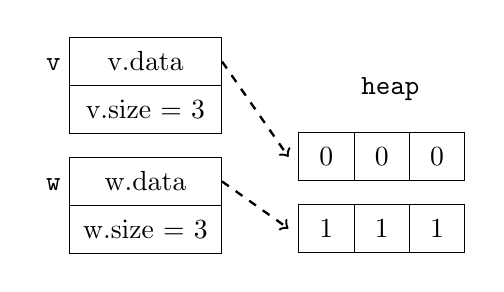
\begin{tikzpicture}[cell/.style={rectangle,draw=black},
            space/.style={minimum height=1.5em,matrix of nodes,row sep=-\pgflinewidth,column sep=-\pgflinewidth,column 1/.style={font=\ttfamily}},text depth=0.5ex,text height=2ex,nodes in empty cells]
            \matrix (foo)[space, column 1/.style={font=\ttfamily},column 2/.style={nodes={cell,minimum width=5.5em}},column 3/.style={nodes={cell,minimum width=2em}},column 4/.style={nodes={cell,minimum width=2em}},column 5/.style={nodes={cell,minimum width=2em}}] 
            {
                {v}   & {v.data}  \\
                                    & {v.size = 3}  \\
            };
             \matrix (bar)[below =0.1em of foo, space, column 1/.style={font=\ttfamily},column 2/.style={nodes={cell,minimum width=5.5em}},column 3/.style={nodes={cell,minimum width=2em}},column 4/.style={nodes={cell,minimum width=2em}},column 5/.style={nodes={cell,minimum width=2em}}] 
            {
                {w}   & {w.data}  \\
                                    & {w.size = 3}  \\
            };

            \matrix (heapname)[right=2em of foo, space, column 1/.style={font=\ttfamily},column 2/.style={font=\ttfamily,nodes={minimum width=5.5em}}] 
            {
                   & {heap}  \\
            };
             \matrix (heap)[below =0.1em of heapname, space, column 1/.style={nodes={cell,minimum width=2em}},column 2/.style={nodes={cell,minimum width=2em}},column 3/.style={nodes={cell,minimum width=2em}},column 4/.style={nodes={cell,minimum width=2em}},column 5/.style={nodes={cell,minimum width=2em}}] 
            {
                       {0} & {0} & {0} \\
            };
             \matrix (heap2)[below =0.1em of heap, space, column 1/.style={nodes={cell,minimum width=2em}},column 2/.style={nodes={cell,minimum width=2em}},column 3/.style={nodes={cell,minimum width=2em}},column 4/.style={nodes={cell,minimum width=2em}},column 5/.style={nodes={cell,minimum width=2em}}]
            {
                       {1} & {1} & {1} \\
            };

             \draw [->, pointer] (foo-1-2.east) to (heap.west);
             \draw [->, pointer] (bar-1-2.east) to (heap2.west);

         \end{tikzpicture}

      \end{column}
      \begin{column}{.5\linewidth}
          \pause
          Ambos objetos comparten los recursos: no hay un ownership claro.
         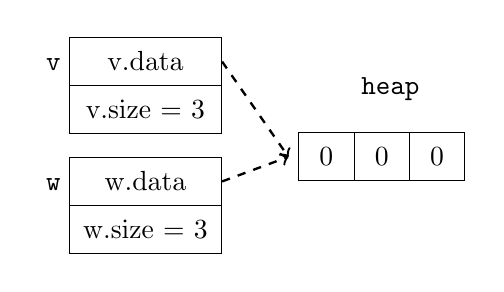
\begin{tikzpicture}[cell/.style={rectangle,draw=black},
            space/.style={minimum height=1.5em,matrix of nodes,row sep=-\pgflinewidth,column sep=-\pgflinewidth,column 1/.style={font=\ttfamily}},text depth=0.5ex,text height=2ex,nodes in empty cells]
            \matrix (foo)[space, column 1/.style={font=\ttfamily},column 2/.style={nodes={cell,minimum width=5.5em}},column 3/.style={nodes={cell,minimum width=2em}},column 4/.style={nodes={cell,minimum width=2em}},column 5/.style={nodes={cell,minimum width=2em}}] 
            {
                {v}   & {v.data}  \\
                                    & {v.size = 3}  \\
            };
             \matrix (bar)[below =0.1em of foo, space, column 1/.style={font=\ttfamily},column 2/.style={nodes={cell,minimum width=5.5em}},column 3/.style={nodes={cell,minimum width=2em}},column 4/.style={nodes={cell,minimum width=2em}},column 5/.style={nodes={cell,minimum width=2em}}] 
            {
                {w}   & {w.data}  \\
                                    & {w.size = 3}  \\
            };

            \matrix (heapname)[right=2em of foo, space, column 1/.style={font=\ttfamily},column 2/.style={font=\ttfamily,nodes={minimum width=5.5em}}] 
            {
                   & {heap}  \\
            };
             \matrix (heap)[below =0.1em of heapname, space, column 1/.style={nodes={cell,minimum width=2em}},column 2/.style={nodes={cell,minimum width=2em}},column 3/.style={nodes={cell,minimum width=2em}},column 4/.style={nodes={cell,minimum width=2em}},column 5/.style={nodes={cell,minimum width=2em}}]
            {
                       {0} & {0} & {0} \\
            };

             \draw [->, pointer] (foo-1-2.east) to (heap.west);
             \draw [->, pointer] (bar-1-2.east) to (heap.west);
         \end{tikzpicture}
      \end{column}
   \end{columns}
\end{frame}

\begin{frame}[fragile]{Constructor por movimiento: transferencia del ownership}
        \begin{lstlisting}[style=normal,firstnumber=1,linebackgroundcolor={%
                 \only<1>{\def\lst@linebgrdcmd####1####2####3{}}%
                 \btLstHLB<2>{6,7}%
                 \btLstHLB<3>{9,10}%
                 \btLstHLB<4>{14,15}%
         }]
struct Vector {
  int *data;
  int size;

  Vector(Vector&& other) {
    this->data = other.data;
    this->size = other.size;

    other.data = nullptr;
    other.size = 0;
  }

  ~Vector() {
      if (data)
          free(data);
  }
};
        \end{lstlisting}
\end{frame}
\note[itemize] {
\item A diferencia de una copia, el constructor por movimiento le roba o mueve los atributos del objeto fuente. 
\item Para marcar el cambio de ownership es necesario modificar al objeto fuente (\lstinline[style=normal]!other!) (por eso no debe ser una constante). Debe dejar de apuntar a los recursos ahora apropiados, de otro modo tendr\'iamos 2 objetos apuntando a un mismo recurso y un bug de memoria a la vuelta de la esquina.
\item Es importante aclarar que luego que el objeto fue movido (\lstinline[style=normal]!other!) debe seguir siendo v\'alido de tal manera que se le puede ejecutar sobre \lstinline[style=normal]!other! el operador asignaci\'on y el destructor. La implementaci\'on de estos dos m\'etodos deben ser acordes como en el ejemplo en donde el destructor pregunta si \lstinline[style=normal]!data == nullptr!
\item C\'omo se implementa la transferencia del ownership depender\'a de cada objeto. En este caso, al poner el puntero \lstinline[style=normal]!data = nullptr! indicamos que no tiene m\'as el ownership del recurso y por lo tanto no tiene que destruirlo.
}

\begin{frame}[fragile]{Pasaje por movimiento}
   \begin{columns}[T]
      \begin{column}{.45\linewidth}
        \begin{lstlisting}[style=normal,firstnumber=1,linebackgroundcolor={%
                 \btLstHLB<1>{3}%
                 \btLstHLB<2>{4,9}%
                 \btLstHLB<3>{12}%
                 \btLstHLR<4>{6}%
                 \btLstHLB<5>{7}%
         }]
// por movimiento
int foo() {
    Vector v(3);
    bar(std::move(v));

    v.get(0); // ??
}

void bar(Vector w) {
  for (int i = 0; /*...*/)
    w.set(i, 1);
}
         \end{lstlisting}

      \end{column}
      \begin{column}{.5\linewidth}
         \begin{tikzpicture}[cell/.style={rectangle,draw=black},
            space/.style={minimum height=1.5em,matrix of nodes,row sep=-\pgflinewidth,column sep=-\pgflinewidth,column 1/.style={font=\ttfamily}},text depth=0.5ex,text height=2ex,nodes in empty cells]
            \matrix (stackname)[space, column 1/.style={font=\ttfamily},column 2/.style={font=\ttfamily,nodes={minimum width=5.5em}}] 
            {
                   & {stack}  \\
            };
            \matrix (foo)[below =0.1em of stackname, space, column 1/.style={font=\ttfamily},column 2/.style={nodes={cell,minimum width=5.5em}},column 3/.style={nodes={cell,minimum width=2em}},column 4/.style={nodes={cell,minimum width=2em}},column 5/.style={nodes={cell,minimum width=2em}}] 
            {
                {\visible<1->{v}}   & {\only<1>{v.data}\only<2-4>{v.data = 0}\only<5>{XX}}  \\
                                    & {\only<1>{v.size = 3}\only<2-4>{v.size = 0}\only<5>{XX}}  \\
            };
             \matrix (bar)[nodevisible on={<2-3>}, below =0.1em of foo, space, column 1/.style={font=\ttfamily},column 2/.style={nodes={cell,minimum width=5.5em}},column 3/.style={nodes={cell,minimum width=2em}},column 4/.style={nodes={cell,minimum width=2em}},column 5/.style={nodes={cell,minimum width=2em}}] 
            {
                {\visible<1->{w}}   & {\only<2>{w.data}\only<3>{XX}}  \\
                                    & {\only<2>{w.size = 3}\only<3>{XX}}  \\
            };

            \matrix (heapname)[right=2em of foo, space, column 1/.style={font=\ttfamily},column 2/.style={font=\ttfamily,nodes={minimum width=5.5em}}] 
            {
                   & {heap}  \\
            };
             \matrix (heap)[nodevisible on={<1-3>}, below =0.1em of heapname, space, column 1/.style={nodes={cell,minimum width=2em}},column 2/.style={nodes={cell,minimum width=2em}},column 3/.style={nodes={cell,minimum width=2em}},column 4/.style={nodes={cell,minimum width=2em}},column 5/.style={nodes={cell,minimum width=2em}}]
            {
                       {\only<1-2>{0}\only<3>{XX}} & {\only<1-2>{0}\only<3>{XX}} & {\only<1-2>{0}\only<3>{XX}} \\
            };

             \draw [->, pointer, arrowvisible on={<1>}] (foo-1-2.east) to (heap.west);
             \draw [->, pointer, arrowvisible on={<2-3>}] (bar-1-2.east) to (heap.west);

         \end{tikzpicture}
        \begin{onlyenv}<1>
        \begin{lstlisting}[style=normal,firstnumber=5]
  Vector(int size) {  // create
    data = malloc(..);
    memset(data, 0 ..);
    this->size = size;
  }
        \end{lstlisting}
        \end{onlyenv}
        \begin{onlyenv}<2>
        \begin{lstlisting}[style=normal,firstnumber=5]
  Vector(Vector&& other) {
    this->data = other.data;
    this->size = other.size;

    other.data = nullptr;
    other.size = 0;
  }
        \end{lstlisting}
        \end{onlyenv}
        \begin{onlyenv}<4>
Use after free!! Pero fue mi culpa. Cuando un objeto es movido solo se le puede invocar el operador asignaci\'on o el destructor, cualquier otra cosa esta mal.
        \end{onlyenv}
        \begin{onlyenv}<5>
Pero no hay un double free.
        \end{onlyenv}
        \begin{visibleenv}<3,5>
        \begin{lstlisting}[style=normal,firstnumber=10]
  ~Vector() { // destroy
     if (data)
        free(data);
  }
        \end{lstlisting}
        \end{visibleenv}
      \end{column}
   \end{columns}
\end{frame}

\begin{frame}[fragile]{Motivaci\'on: retorno de un Socket}{}
Por referencia? \only<2->{Ineficiente o viola RAII}
        \begin{lstlisting}[style=normal,firstnumber=1]
Socket s;
acep.accept(s);
        \end{lstlisting}

        \begin{lstlisting}[style=normal,firstnumber=10]
void accept(Socket &s) {
    close(s.fd);
    s.fd = ::accept(/*...*/); // accept de C
}
        \end{lstlisting}

        \pause
        \pause
Usando el heap? \only<4->{Y si nos olvidamos del \lstinline[style=normal]!delete!?}
        \begin{lstlisting}[style=normal,firstnumber=1]
Socket *s = acep.accept();
        \end{lstlisting}
        \begin{lstlisting}[style=normal,firstnumber=10]
Socket* accept() {
    int fd = ::accept(/*...*/); // accept de C
    return new Socket(fd);
}
        \end{lstlisting}
        \pause
        \pause
Retornar una copia? \only<6->{Tiene sentido? Simplemente No.}

\end{frame}
\note[itemize] {
\item Por referencia: Ineficiente, creamos un \lstinline[style=normal]!fd! para cerrarlo y asignar otro.
\item Por referencia: O bien, el constructor de \lstinline[style=normal]!Socket! no abren ningun \lstinline[style=normal]!fd! (pero entonces no ser\'ian RAII)
\item Por heap: El constructor \lstinline[style=normal]!Socket(int)! debe ser privado.
\item Por heap: Perdemos la ventaja de usar el stack.
}

\begin{frame}[fragile]{Soluci\'on?: Mover el Socket!!}{}
Por movimiento!
        \begin{lstlisting}[style=normal,firstnumber=1]
Socket s = acep.accept();
        \end{lstlisting}
        \begin{lstlisting}[style=normal,firstnumber=10]
Socket accept() {
    int fd = ::accept(/*...*/); // accept de C
    return std::move(Socket(fd));
}
        \end{lstlisting}
   \begin{itemize}
	   \item El constructor \lstinline[style=normal]!Socket(int)! debe ser privado.
	   \item El socket creado dentro del m\'etodo \lstinline[style=normal]!accept! es movido hacia afuera.
	   \item Todos los objetos involucrados viven en el stack y por lo tanto se destruyen autom\'aticamente.
   \end{itemize}
\end{frame}
\note[itemize] {
\item El m\'etodo \lstinline[style=normal]!accept! retorna un nuevo objeto \lstinline[style=normal]!Socket!.
\item El m\'etodo no quiere tener el ownership del nuevo socket creado, quiere moverlo y darselo a quien lo llam\'o.
\item En C y en C++ antes del est\'andar C++11 no hab\'ia otra forma que o pasaje por referencia (lo que implicaba que hab\'ia que construir previamente un \lstinline[style=normal]!Socket! dummy para luego inicializarlo correctamente dentro de \lstinline[style=normal]!accept!) o bien retornarlo usando el heap (perdiendo el beneficio de ser RAII).
\item El compilador puede deducir que el objeto \lstinline[style=normal]!accepted! se lo desea mover. Usar \lstinline[style=normal]!std::move! para hacerlo expl\'icito.
}


\begin{frame}[fragile]{Otro ejemplo: pasando objetos a un hilo}{}
        \begin{lstlisting}[style=normal,firstnumber=10]
std::thread aceptar_un_cliente(Socket &aceptador) {
    Socket skt_cliente = aceptador.accept();

    // movimiento de un socket, todo ok
    std::thread t {manejador_del_cliente,
                   std::move(skt_cliente)};

    return std::move(t);
} // <--el socket skt_cliente se destruye, pero como se movio
  // no deberia pasar nada (siempre que se implemente el
  // constructor por movimiento y el destructor acorde!)

        \end{lstlisting}
\end{frame}
\note[itemize] {
\item La funci\'on crea un nuevo socket \lstinline[style=normal]!skt_cliente! y se lo pasa a un hilo para que lo procese en paralelo.
\item El fin de \lstinline[style=normal]!aceptar_un_cliente! no implica que el socket \lstinline[style=normal]!skt_cliente! se deba cerrar: el lifetime del objeto deber\'ia estar atado al del hilo.
\item No podemos pasar una copia ya que no tiene sentido copiar un socket.
\item Tampoco una referencia ya que el objeto \lstinline[style=normal]!skt_cliente! vive en el stack frame de \lstinline[style=normal]!aceptar_un_cliente! y se destruir\'a al finalizar esta.
\item En C y en C++ antes del est\'andar C++11 no hay otra alternativa que poner el socket \lstinline[style=normal]!skt_cliente! en el heap perdiendo los beneficios RAII. En C++11 se lo mueve directamente.
\item Lo mismo ocurre con el retorno del objeto thread \lstinline[style=normal]!t!.
}

\section{Asignaci\'on}
\subsection{Asignaci\'on por copia}
\begin{frame}[fragile]{Asignaci\'on}
        \begin{lstlisting}[style=normal,firstnumber=1,linebackgroundcolor={%
                 \btLstHLB<1>{1-3,9}%
                 \btLstHLB<2>{7}%
         }]
Vector f(Vector v) {
  Vector a(v);
  Vector b = v;

  Vector c(5);

  c = v;

  return v;
}
        \end{lstlisting}
\end{frame}
\note[itemize] {
\item En la l\'inea 1 se recibe por copia un vector al que llamaremos \lstinline[style=normal]!v!.
\item En la l\'inea 2 y 3 se crean 2 vectores m\'as copiandose de \lstinline[style=normal]!v!, ambos llaman al constructor por copia.
\item En la l\'inea 9 se retorna un vector por copia tambi\'en salvo que \lstinline[style=normal]!Vector! implemente el constructor por movimiento en cuyo caso \lstinline[style=normal]!v! se mueve y no se copia.
\item En la l\'inea 7 sucede algo distinto. El vector \lstinline[style=normal]!c! copia el contenido del vector \lstinline[style=normal]!v!. Pero el objeto \lstinline[style=normal]!c! ya estaba creado asi que en vez de llamar al constructor por copia llama al operador asignaci\'on por copia.
}

\begin{frame}[fragile]{Asignaci\'on por copia: un objeto creado copiando de otro}
        \begin{lstlisting}[style=normal,firstnumber=1,linebackgroundcolor={%
                 \only<1>{\def\lst@linebgrdcmd####1####2####3{}}%
                 \btLstHLB<2>{10,11}%
                 \btLstHLB<3>{13-15}%
                 \btLstHLB<4>{6-8}%
         }]
struct Vector {
  int *data;
  int size;

  Vector& operator=(const Vector &other) {
    if (this == &other) {
      return *this; // other is myself!
    }

    if (this->data)
        free(this->data);

    this->data = (int*)malloc(other.size*sizeof(int));
    this->size = other.size;
    memcpy(this->data, other.data; this->size);

    return *this;
  }
};
        \end{lstlisting}
\end{frame}
\note[itemize] {
\item Para copiar el contenido de un objeto en otro ya creado se usa el operador asignaci\'on.
\item Como el objeto \lstinline[style=normal]!this! ya esta creado, debemos recordar que todos sus atributos estan ya creados: no podemos cambiar ninguno de sus atributos constantes.
\item Validar que no nos hayan quitado el ownership de nuestros recursos.
\item Todos los objetos en C++ son copiables por asignaci\'on asi que si un objeto no implementa la sobrecarga del operador asignaci\'on, C++ le creara una implementaci\'on por default que hara una copia bit a bit naive.
\item Tambi\'en es posible que nos asignemos a nosotros mismos (haciendo \lstinline[style=normal]!vec = vec;!). Debemos programar el operador asignaci\'on de tal forma que evite copiarse a si mismo.
\item El operador asignaci\'on no es el \'unico operador que se puede sobrecargar. Ya veremos otros y en m\'as detalle en las pr\'oximas clases.
}

\subsection{Asignaci\'on por movimiento}
\begin{frame}[fragile,plain]{Asignaci\'on por movimiento}{}
        \begin{lstlisting}[style=normal,firstnumber=1]
struct Vector {
  int *data;
  int size;

  Vector& operator=(Vector&& other) {
    if (this == &other) {
      return *this; // other is myself!
    }

    if (this->data)
        free(this->data);

    this->data = other.data;
    this->size = other.size;

    other.data = nullptr;
    other.size = 0;

    return *this;
  }
};
        \end{lstlisting}
\end{frame}

\begin{frame}[fragile]{Ej Asignaci\'on por movimiento: swap de objetos}{}
        \begin{lstlisting}[style=normal,firstnumber=10]
void swap(Vector& a, Vector& b) {
    Vector t = a;  // copia (constructor)
    a = b;  // copia (asignacion)
    b = t;  // copia (asignacion)
}
        \end{lstlisting}
        \begin{lstlisting}[style=normal,firstnumber=10]
void swap(Vector& a, Vector& b) {
    Vector t = std::move(a); // a se mueve a t (constructor)
    a = std::move(b); // b se mueve a a (asignacion)
    b = std::move(t); // t se mueve a b (asignacion)
}
        \end{lstlisting}
\end{frame}


%\begin{frame}[plain, fragile]{}{}
%   \begin{columns}[T]
%      \begin{column}{.5\linewidth}
%         \begin{lstlisting}[style=normal,numbers=none]
%void _copy(const Vector &other) {
%  data = malloc(other.size*
%                sizeof(int));
%  size = other.size;
%  memcpy(data, other.data, size);
%}
%
%Vector(const Vector &other) {
%  _copy(other);
%}
%
%Vector&
%operator=(const Vector &other) {
%  if (this == &other)
%    return *this;
%
%  !data || free(data);
%  _copy(other);
%  return *this;
%}
%
%         \end{lstlisting}
%      \end{column}
%      \begin{column}{.45\linewidth}
%         \begin{lstlisting}[style=normal,numbers=none]
%void _move(Vector&& other) {
%  data = other.data;
%  size = other.size;
%  other.data = nullptr;
%  other.size = 0;
%}
%
%Vector(Vector&& other) {
%  _move(other);
%}
%
%Vector&
%operator=(Vector&& other) {
%  if (this == &other)
%    return *this;
%
%  !data || free(data);
%  _move(other);
%  return *this;
%}
%         \end{lstlisting}
%      \end{column}
%   \end{columns}
%\end{frame}

\section{Objetos no copiables}
\subsection*{Objetos no copiables}
\begin{frame}[fragile]{ Objetos no copiables}{}
        \begin{lstlisting}[style=normal,firstnumber=1]
struct File {
  public:
  File copy(const char *to_where) { ... }

  private:
  File(const File &other) = delete;
  File& operator=(const File &other) = delete;

};
        \end{lstlisting}
\end{frame}
\note[itemize] {
\item En C++11 podemos decir que tanto el constructor por copia como el de asignaci\'on estan borrados (\lstinline[style=normal]!delete!). Si en algun momento intentamos hacer una copia el compilador dara un error.
\item Pero si trabajamos en C++98, debemos usar algun workaround: declarar y definir el constructor por copia y el operador asignaci\'on y que su implementaci\'on sea fallar (lanzar una excepci\'on). El intento fallido de copia se detecta en runtime.
\item Otra forma seria declarar pero no definir ni el constructor por copia ni el operador asignaci\'on y hacerlos privados. El intento fallido de copia se detecta en tiempo de compilaci\'on y linkeo.
}

\begin{frame}[fragile]{Resumen}
   \begin{itemize}
       \item Implementar el constructor y destructor con el idiom RAII: el objeto se hacer cargo (ownership) del recurso.
       \item Implementar constructor y asignaci\'on por movimiento.
       \item Hacer que el objeto no sea copiable.
       \begin{itemize}
            \item Si se necesita copiar un objeto implementar un m\'etodo \lstinline[style=normal]!copy!. Si se quiere copiar, que sea una llamada expl\'icita y no autom\'atica.
            \item En \'ultima instancia, implementar el constructor y asignaci\'on por copia.
       \end{itemize}
   \end{itemize}
\end{frame}

\appendix
\section<presentation>*{\appendixname}
\subsection<presentation>*{Referencias}

\begin{frame}[allowframebreaks]
   \frametitle<presentation>{Referencias}

   \begin{thebibliography}{10}

         \beamertemplatebookbibitems
         % Start with overview books.

      \bibitem{Stroustrup}
         Bjarne Stroustrup.
         \newblock {\em The C++ Programming Language}.
         \newblock Addison Wesley, Fourth Edition.

   \end{thebibliography}
\end{frame}

\end{document}


